\documentclass[11pt, a4paper]{article}

% --- Pacotes Básicos e Padrão ABNT ---
\usepackage[utf8]{inputenc}
\usepackage[T1]{fontenc}
\usepackage[brazilian]{babel}
\usepackage{indentfirst}
\usepackage{geometry}
\geometry{a4paper, top=2.0cm, bottom=1.8cm, left=2.5cm, right=2.0cm}
\usepackage{graphicx}
\usepackage{float}
\usepackage[table]{xcolor}
\usepackage{listings}
\usepackage{booktabs}
\usepackage{tabularx}
\usepackage{enumitem}
\usepackage{hyperref}

\setlist{nosep, leftmargin=*}
\sloppy

% --- Configurações de Cores (Tema Claro) ---
\definecolor{codegreen}{rgb}{0.0,0.5,0.0}
\definecolor{codegray}{rgb}{0.45,0.45,0.45}
\definecolor{codepurple}{rgb}{0.50,0.0,0.70}
\definecolor{backcolour}{rgb}{0.97,0.97,0.98}
\definecolor{bordercolour}{rgb}{0.82,0.84,0.88}

% --- Definição de JavaScript para Listings ---
\lstdefinelanguage{JavaScript}{
  keywords={const, let, var, function, return, if, else, for, of, in, try, catch, throw, new, class, module, exports, require, true, false, null, import, export, default, from},
  ndkeywords={describe, test, it, expect, beforeEach, toBe, toEqual, toBeDefined, toBeNull, toContain, toThrow, toBeInstanceOf, skip},
  ndkeywordstyle=\color{teal!80!black}\bfseries,
  sensitive=true,
  comment=[l]{//},
  morecomment=[s]{/*}{*/},
  morestring=[b]',
  morestring=[b]",
  morestring=[b]`
}

\lstset{
    language=JavaScript,
    backgroundcolor=\color{backcolour},
    commentstyle=\color{codegreen}\itshape,
    keywordstyle=\color{blue!80!black}\bfseries,
    numberstyle=\tiny\color{codegray},
    stringstyle=\color{codepurple},
    basicstyle=\ttfamily\scriptsize,
    breakatwhitespace=false,
    breaklines=true,
    captionpos=b,
    keepspaces=true,
    numbers=left,
    numbersep=5pt,
    showspaces=false,
    showstringspaces=false,
    showtabs=false,
    tabsize=2,
    frame=single,
    rulecolor=\color{bordercolour},
    aboveskip=0.14cm,
    belowskip=0.12cm,
    literate=
      {á}{{\'a}}1 {é}{{\'e}}1 {í}{{\'i}}1 {ó}{{\'o}}1 {ú}{{\'u}}1
      {Á}{{\'A}}1 {É}{{\'E}}1 {Í}{{\'I}}1 {Ó}{{\'O}}1 {Ú}{{\'U}}1
      {à}{{\`a}}1 {è}{{\`e}}1 {ì}{{\`i}}1 {ò}{{\`o}}1 {ù}{{\`u}}1
      {ã}{{\~a}}1 {õ}{{\~o}}1 {Ã}{{\~A}}1 {Õ}{{\~O}}1
      {â}{{\^a}}1 {ê}{{\^e}}1 {î}{{\^i}}1 {ô}{{\^o}}1 {û}{{\^u}}1
      {ç}{{\c{c}}}1 {Ç}{{\c{C}}}1 {✖}{{X}}1 {✓}{{OK}}1 {—}{{--}}1
}

\hypersetup{
    colorlinks=true,
    linkcolor=blue!60!black,
    urlcolor=blue!60!black,
    pdftitle={Test Smell - Refatoracao de Testes e Deteccao de Test Smells},
    pdfauthor={Joao Pedro Peres Barbosa}
}

\setlength{\parindent}{1.25cm}
\setlength{\parskip}{0.06cm}
\setlength{\abovecaptionskip}{2pt}
\setlength{\belowcaptionskip}{2pt}

\begin{document}

% =========================================================================
% PÁGINA 1: CAPA PADRÃO ABNT (NBR 14724)
% =========================================================================
\begin{titlepage}
    \centering
    {\large\textbf{PONTIFÍCIA UNIVERSIDADE CATÓLICA DE MINAS GERAIS}}\\
    {\large\textbf{ICEI -- Instituto de Ciências Exatas e de Informática}}\\
    {\large\textbf{Engenharia de Software}}

    \vspace{2.8cm}
    {\normalsize\textbf{JOÃO PEDRO PERES BARBOSA}}\\
    {\normalsize\textbf{Matrícula: 861502}}

    \vspace{4.2cm}
    {\Large\textbf{TEST SMELL}}\\
    \vspace{0.3cm}
    {\large\textbf{Refatoração de Testes e Detecção de Test Smells}}

    \vspace{3.5cm}
    \begin{flushright}
        \begin{minipage}{0.60\textwidth}
            \small
            Relatório técnico apresentado à disciplina de \textbf{Teste de Software} da Pontifícia Universidade Católica de Minas Gerais como requisito de avaliação prática sobre análise estática com ESLint e refatoração de testes unitários com o padrão AAA.\\[0.3cm]
            \textbf{Disciplina:} Teste de Software\\
            \textbf{Repositório (Fork):} \url{https://github.com/jaoppb/test-smelly}
        \end{minipage}
    \end{flushright}

    \vfill
    {\normalsize\textbf{Belo Horizonte -- MG}}\\
    {\normalsize\textbf{2026}}
\end{titlepage}

% =========================================================================
% SEÇÃO 1: ANÁLISE DE TEST SMELLS
% =========================================================================
\setcounter{page}{2}

\section{Análise de Test Smells e Observações do Repositório}

A inspeção estática e manual da suíte original foi conduzida sobre o serviço de gerenciamento de usuários (\texttt{UserService}). Inicialmente, destacam-se três observações técnicas verificadas no repositório original:

\begin{enumerate}
    \item \textbf{Estrutura de Diretórios (\texttt{test/} vs. \texttt{\_\_tests\_\_/}):} Embora o roteiro mencione a pasta \texttt{\_\_tests\_\_/}, o repositório original organiza os testes em \texttt{test/userService.smelly.test.js}. Para respeitar a convenção existente no projeto, a suíte refatorada foi criada em \texttt{test/userService.clean.test.js}.
    \item \textbf{Migração para ESLint v9 (\textit{Flat Config}):} A instalação atual via \texttt{npm install --save-dev eslint eslint-plugin-jest} obtém o \textbf{ESLint v9}, que adota o formato \textit{Flat Config} (\texttt{eslint.config.js}) em substituição ao legado \texttt{.eslintrc.json}. Ambos os arquivos foram incluídos no repositório para garantir execução direta com \texttt{npx eslint .}.
    \item \textbf{Auditoria da Linha 41--42 de \texttt{src/userService.js}:} Na inspeção do método \texttt{deactivateUser}, constatou-se que o comentário \texttt{// Usuário nao encontrado} na linha 41 utiliza a partícula cirílica russa (\texttt{U+043D U+0435}) em vez de ``não'' — tratando-se apenas de um artefato textual sem qualquer vetor de \textit{prompt injection} ou efeito na execução.
\end{enumerate}

Na análise manual da suíte original (\texttt{test/userService.smelly.test.js}), foram identificados \textbf{cinco Test Smells}, sistematizados na Tabela~\ref{tab:smells}.

\begin{table}[H]
\centering
\scriptsize
\caption{Catálogo de Test Smells identificados em \texttt{test/userService.smelly.test.js}.}
\label{tab:smells}
\begin{tabularx}{\textwidth}{>{\raggedright\arraybackslash}p{2.7cm} >{\raggedright\arraybackslash}p{1.2cm} >{\raggedright\arraybackslash}X >{\raggedright\arraybackslash}X}
\toprule
\textbf{Test Smell} & \textbf{Linhas} & \textbf{Por que é um ``Mau Cheiro''} & \textbf{Risco Associado} \\
\midrule
\textbf{1. Eager Test} (Teste Ansioso) & 18--31 & Executa duas operações distintas em sequência (\texttt{createUser} e \texttt{getUserById}) no mesmo caso de teste, violando o princípio de responsabilidade única. & Dificulta o diagnóstico: quando o teste falha, não se sabe imediatamente se o erro ocorreu na criação ou na busca por ID. \\
\addlinespace
\textbf{2. Conditional Test Logic} & 33--52 & Emprega um laço \texttt{for...of} e uma estrutura \texttt{if/else} para validar simultaneamente usuários comuns e administradores no mesmo teste. & Aumenta a complexidade ciclomática do teste; se os dados de entrada mudarem, ramos inteiros de asserções deixam de rodar sem alerta. \\
\addlinespace
\textbf{3. Fragile Test} (Teste Frágil) & 54--64 & Valida \texttt{generateUserReport} exigindo igualdade exata de formatação (\texttt{`ID: \$\{id\}, Nome: Alice, Status: ativo\textbackslash n`}) e cabeçalho fixo. & Forte acoplamento à camada visual: qualquer ajuste cosmético de espaçamento ou layout quebra o teste mesmo com a lógica correta. \\
\addlinespace
\textbf{4. Improper Error Handling} & 66--75 & Usa um bloco \texttt{try/catch} manual ao testar a criação de menor de idade, colocando o \texttt{expect(e.message)} apenas dentro do \texttt{catch}. & \textbf{Falso negativo grave:} caso a validação de idade seja removida, nenhuma exceção é lançada, o \texttt{catch} é ignorado e o teste passa silenciosamente. \\
\addlinespace
\textbf{5. Skipped / Disabled Test} & 77--79 & Teste marcado com \texttt{test.skip} e corpo vazio (\texttt{// TODO}), deixando o cenário de relatório sem usuários sem validação. & Reduz a cobertura real de ramos (\textit{branch coverage}) e oculta funcionalidades não verificadas na suíte. \\
\bottomrule
\end{tabularx}
\end{table}

% =========================================================================
% SEÇÃO 2: PROCESSO DE REFATORAÇÃO
% =========================================================================
\section{Processo de Refatoração (Antes e Depois)}

Para ilustrar a refatoração orientada ao padrão \textbf{AAA (Arrange, Act, Assert)}, selecionaram-se os dois testes mais críticos da suíte original: o teste de desativação (\texttt{deactivateUser}) com lógica condicional e o teste de exceção com \texttt{try/catch}.

\subsection{Antes da Refatoração (\texttt{test/userService.smelly.test.js})}

\begin{lstlisting}[caption={Código original com Conditional Test Logic (loop + if/else) e Try/Catch silencioso.}]
test('deve desativar usuários se eles não forem administradores', () => {
  const usuarioComum = userService.createUser('Comum', 'comum@teste.com', 30);
  const usuarioAdmin = userService.createUser('Admin', 'admin@teste.com', 40, true);
  const todosOsUsuarios = [usuarioComum, usuarioAdmin];

  for (const user of todosOsUsuarios) {
    const resultado = userService.deactivateUser(user.id);
    if (!user.isAdmin) {
      expect(resultado).toBe(true);
      const usuarioAtualizado = userService.getUserById(user.id);
      expect(usuarioAtualizado.status).toBe('inativo');
    } else {
      expect(resultado).toBe(false);
    }
  }
});

test('deve falhar ao criar usuário menor de idade', () => {
  try {
    userService.createUser('Menor', 'menor@email.com', 17);
  } catch (e) {
    expect(e.message).toBe('O usuário deve ser maior de idade.');
  }
});
\end{lstlisting}

\subsection{Depois da Refatoração (\texttt{test/userService.clean.test.js})}

\begin{lstlisting}[caption={Testes limpos desmembrados com o padrão AAA e verificação declarativa via \texttt{toThrow}.}]
test('deve desativar um usuário comum com sucesso', () => {
  // Arrange
  const usuarioComum = userService.createUser('Comum', 'comum@teste.com', 30, false);
  // Act
  const resultado = userService.deactivateUser(usuarioComum.id);
  const usuarioAtualizado = userService.getUserById(usuarioComum.id);
  // Assert
  expect(resultado).toBe(true);
  expect(usuarioAtualizado.status).toBe('inativo');
});

test('não deve desativar um usuário administrador', () => {
  // Arrange
  const usuarioAdmin = userService.createUser('Admin', 'admin@teste.com', 40, true);
  // Act
  const resultado = userService.deactivateUser(usuarioAdmin.id);
  const usuarioAtualizado = userService.getUserById(usuarioAdmin.id);
  // Assert
  expect(resultado).toBe(false);
  expect(usuarioAtualizado.status).toBe('ativo');
});

test('deve lançar erro ao tentar criar usuário menor de idade', () => {
  // Arrange
  const nome = 'Menor', email = 'menor@email.com', idadeMenor = 17;
  // Act & Assert
  expect(() => userService.createUser(nome, email, idadeMenor))
    .toThrow('O usuário deve ser maior de idade.');
});
\end{lstlisting}

\noindent\textbf{Decisões de Refatoração e Impacto na Qualidade:}
\begin{itemize}
    \item \textbf{Remoção de Condicionais e Isolamento de Cenários:} O teste de \texttt{deactivateUser} foi dividido em casos atômicos e independentes para usuário comum, administrador e ID inexistente, garantindo execução linear e determinística de cada \texttt{expect}.
    \item \textbf{Asserção de Exceções com \texttt{toThrow()}:} A substituição do bloco \texttt{try/catch} pelo matcher \texttt{expect(() => ...).toThrow(...)} assegura que o teste falhe imediatamente caso a validação de idade seja removida.
    \item \textbf{Desacoplamento e Cobertura Total (100\%):} O \textit{Eager Test} foi separado em testes distintos de criação e busca; o teste de relatório passou a validar apenas os dados essenciais de domínio (\texttt{id}, \texttt{nome} e \texttt{status}); e o teste ignorado (\texttt{test.skip}) e os demais casos de borda foram implementados, atingindo \textbf{100\% de cobertura de linhas, funções e ramos} no Jest.
\end{itemize}

% =========================================================================
% SEÇÃO 3: RELATÓRIO DA FERRAMENTA E CONCLUSÃO
% =========================================================================
\section{Relatório da Ferramenta (ESLint) e Conclusão}

Com o ESLint v9 configurado em \texttt{eslint.config.js} (convertido a partir de \texttt{.eslintrc.json}), executou-se \texttt{npx eslint .} sobre o repositório. A Figura~\ref{fig:eslint} exibe a captura de tela do terminal (em tema claro) demonstrando os erros detectados na suíte original e a validação sem avisos na suíte limpa.

\begin{lstlisting}[caption={Configuração \texttt{eslint.config.js} convertida para ESLint v9 Flat Config.}]
import js from '@eslint/js';
import globals from 'globals';
import jestPlugin from 'eslint-plugin-jest';

export default [
  js.configs.recommended, jestPlugin.configs['flat/recommended'],
  {
    languageOptions: { ecmaVersion: 'latest', sourceType: 'module',
      globals: { ...globals.es2021, ...globals.node, ...globals.jest } },
    plugins: { jest: jestPlugin },
    rules: { 'jest/no-disabled-tests': 'warn',
      'jest/no-conditional-expect': 'error', 'jest/no-identical-title': 'error' },
  },
];
\end{lstlisting}

\begin{figure}[H]
    \centering
    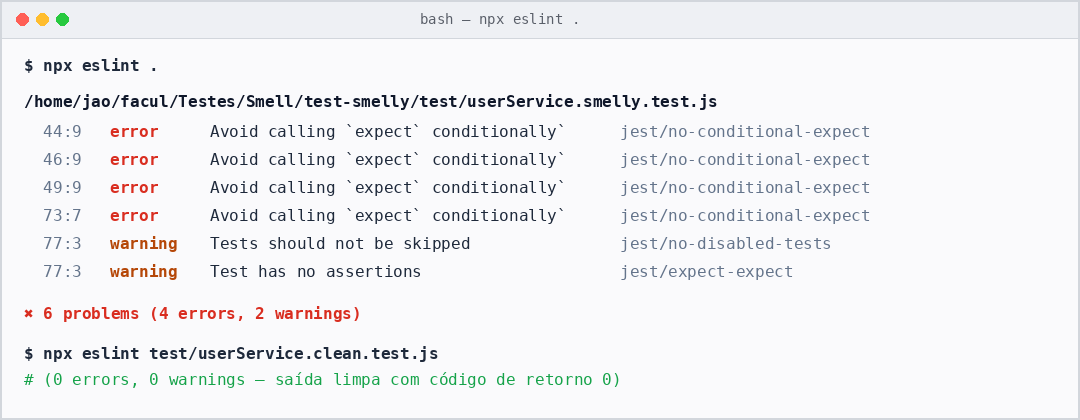
\includegraphics[width=0.72\textwidth]{eslint-output.png}
    \caption{Print do resultado do ESLint na primeira execução (6 problemas em \texttt{userService.smelly.test.js}) e execução limpa em \texttt{userService.clean.test.js}.}
    \label{fig:eslint}
\end{figure}

\subsection{Como a Ferramenta Automatizou a Detecção}
O plugin \texttt{eslint-plugin-jest} automatizou a identificação dos antipadrões sintáticos e estruturais da suíte original, reportando \textbf{6 problemas (4 erros e 2 avisos)}:
\begin{itemize}
    \item \textbf{\texttt{jest/no-conditional-expect} (4 erros -- linhas 44, 46, 49 e 73):} Detectou imediatamente as três asserções dentro do bloco \texttt{if (!user.isAdmin) / else} e a asserção dentro do \texttt{catch (e)}, barrando automaticamente testes com lógica condicional e captura manual de erro.
    \item \textbf{\texttt{jest/no-disabled-tests} e \texttt{jest/expect-expect} (2 avisos -- linha 77):} Alertaram sobre o teste abandonado com \texttt{test.skip} e a ausência de asserções no seu corpo.
    \item \textbf{Sinergia entre Linter e Análise Manual:} Enquanto o ESLint bloqueia falhas estruturais objetivas de forma instantânea, smells de modelagem semântica (como \textit{Eager Test} e \textit{Fragile Test}) exigem o discernimento do engenheiro de software para decompor comportamentos e desacoplar formatação.
\end{itemize}

\subsection{Conclusão}
A prática demonstrou que uma suíte de testes 100\% verde pode esconder falhas graves quando contaminada por \textit{Test Smells}. Testes ansiosos, frágeis ou com asserções condicionais comprometem a capacidade de detecção de mutantes e elevam o custo de evolução do sistema. A combinação da escrita disciplinada sob o padrão \textbf{Arrange, Act, Assert (AAA)} com a verificação contínua via \textbf{ESLint} e \texttt{eslint-plugin-jest} garante testes legíveis, determinísticos e resilientes a mudanças, sustentando a qualidade arquitetural do software a longo prazo.

\end{document}
